% รายงานอัลกอริทึม Detour Steer ฉบับภาษาไทย (Thai version of 660610840_DetourSteer_EN.tex)
% Build (XeLaTeX, Thai font):  xelatex 660610840_DetourSteer.tex   (run twice, inside algorithm_sim/docs)

\documentclass[11pt,a4paper]{article}

\usepackage[top=1.5cm,bottom=1.5cm,left=1.9cm,right=1.9cm]{geometry}
\usepackage{amsmath}
\usepackage{amssymb}
\usepackage{mathpazo}
\usepackage{fontspec}
\setmainfont{Leelawadee UI}[Scale=0.92, BoldFont={Leelawadee UI Bold}]
\setmonofont{Consolas}[Scale=0.9]
\XeTeXlinebreaklocale "th"
\XeTeXlinebreakskip = 0pt plus 1pt
\linespread{1.12}
\usepackage{needspace}
\usepackage{booktabs}
\usepackage[linesnumbered,lined]{algorithm2e}
\usepackage{graphicx}
\usepackage{url}
\usepackage{listings}
\usepackage{xcolor}
\usepackage[hidelinks]{hyperref}
\lstset{basicstyle=\ttfamily\scriptsize,numbers=left,numberstyle=\tiny\color{gray},frame=single,breaklines=true,columns=fullflexible,keepspaces=true,showstringspaces=false,commentstyle=\color{gray}}

% ---------------------------------------------------------------- styling ---
\RestyleAlgo{boxed}
\SetAlgoNlRelativeSize{-1}
\newcommand{\algcommentfont}[1]{\footnotesize\textnormal{#1}}
\SetCommentSty{algcommentfont}
\SetKwComment{tcp}{/\kern-0.12em/\ }{}
\SetFuncSty{textit}
\SetArgSty{textnormal}

\newcommand{\algohead}[3][62mm]{%
  \Needspace*{#1}%
  \par\addvspace{2mm}%
  \noindent\rule{\linewidth}{1.1pt}\par
  \vspace{1.4mm}%
  \noindent\textbf{อัลกอริทึม #2:} #3\par
  \vspace{1.4mm}%
  \noindent\rule{\linewidth}{0.5pt}\par
  \vspace{0.8mm}%
}
\newcommand{\algofoot}{%
  \par\vspace{0.8mm}%
  \noindent\rule{\linewidth}{1.1pt}\par
  \addvspace{4.5mm}%
}

% ------------------------------------------------------------- keywords -----
\SetKwProg{Pro}{Procedure :}{}{end}
\SetKwFunction{FOpt}{OptimalDetourAngle}
\SetKwFunction{FPlan}{PlanLeg}
\SetKwFunction{FDetourSteer}{DetourSteer}
\SetKwFunction{FFollow}{FollowRouteDetour}
\SetKwFunction{FCwError}{SteeringError}
\SetKwFunction{FInTol}{InTolerance}
\SetKwFunction{FBearing}{Bearing}
\SetKwFunction{FDrive}{Drive}
\SetKwFunction{FStop}{Stop}
\SetKwFunction{FPos}{MeasurePosition}
\SetKwFunction{FHead}{MeasureHeading}
\SetKwFunction{FSteerOne}{SteerOneWay}
\SetKwFunction{FDriveReaim}{DriveReaim}
\SetKw{KwDisplay}{แสดง}
\SetKw{KwAnd}{and}
\SetKw{KwOr}{or}
\SetKw{KwNone}{None}

\pagestyle{empty}

\begin{document}

\begin{flushright}
  {\small\bfseries Phuthiphong Wongchantib 660610840}
\end{flushright}
\vspace{-2mm}

\begin{center}
  {\large\bfseries หุ่นยนต์ที่เลี้ยวได้ทางเดียว (ทวนเข็มนาฬิกา) --- อัลกอริทึม Detour Steer}\\[1.2mm]
  วิ่งไปก่อน เลี้ยวให้น้อยลง แล้วค่อยเข้าเป้า
\end{center}
\vspace{1mm}

\noindent{\small\textbf{ตัวหุ่น} มีมอเตอร์ DC ตัวเดียว หมุนทางหนึ่งเป็นการ\emph{เลี้ยว}ชุดล้อ
ได้\emph{ทวนเข็มนาฬิกาเท่านั้น} (มีคลัตช์ทางเดียว) หมุนอีกทางเป็นการ\emph{วิ่ง}ไปข้างหน้า
หุ่นจึงเลี้ยวกับวิ่งพร้อมกันไม่ได้
วิธีเดิมคือเลี้ยวตรงไปหาเป้าก่อนแล้วค่อยวิ่ง ถ้าเป้าอยู่ทาง\emph{ขวา}นิดเดียว ($\varphi$ ใกล้ $360^\circ$)
ล้อต้องหมุนเกือบรอบ
\textbf{แนวคิด} เส้นตรงสองช่วงที่ทิศต่างกันเกิน $180^\circ$ ไปถึงได้\emph{ทุก}ทิศ
หุ่นจึงเลือกได้ว่าจะวิ่งตรงไปก่อน $a$ เมตร เลี้ยวแค่ $\beta^\ast$ ($180^\circ < \beta^\ast < \varphi$)
แล้ววิ่งอีก $b$ เมตรถึงเป้า มุม $\beta^\ast$ ที่ดีที่สุดมีสูตรปิดคำนวณได้ทันที
มุมทุกมุมวัดทวนเข็มนาฬิกาจากแกน $+x$ ;
$\omega$ = ความเร็วเลี้ยว, $v$ = ความเร็ววิ่ง, $t_s$ = เวลารอล้อนิ่ง,
$t_b$ = เวลาหยุดเปลี่ยนจากวิ่งเป็นเลี้ยว, $tol$ = ค่าคลาดเคลื่อนที่ยอมได้, $r_{goal}$ = รัศมีถือว่าถึงเป้า
\textbf{บนหุ่นจริง} (\texttt{mor\_luam}, ESP32) ชุดล้อเลี้ยวทวนเข็มเมื่อมองจากด้านบน ตรงกับระบบมุมในหน้านี้
(ชื่อฟังก์ชัน cwErrorDeg ในเฟิร์มแวร์เป็นชื่อเก่า แต่ค่าที่ได้คือมุมทวนเข็ม)
อัลกอริทึม 1.1--1.5 คือการวางแผน ส่วน 1.6--1.7 คือวิธีที่หุ่นเลี้ยวและวิ่งแต่ละช่วงจริง}
\vspace{1mm}

\section*{ส่วนที่ 1 อัลกอริทึม: ทำไมเร็วกว่า (พิสูจน์ และซิมอุดมคติ)}
% ============================================================ Algorithm 1.1 ==
\algohead{1.1}{ฟังก์ชันช่วยเรื่องมุม (ทวนเข็มนาฬิกา)}
{\small
\begin{algorithm}[H]
\Pro(\tcp*[f]{มุมทวนเข็มของทิศ $(\Delta x, \Delta y)$}){\FBearing{$\Delta x$, $\Delta y$}}{
  \KwRet{$\operatorname{atan2}(\Delta y, \Delta x) \bmod 2\pi$}\;
}
\BlankLine
\Pro(\tcp*[f]{ล้อต้องเลี้ยวทวนเข็มอีกเท่าไร: $0 \ldots 2\pi$}){\FCwError{$\theta$, $h$}}{
  \KwRet{$(\theta - h) \bmod 2\pi$}\;
}
\BlankLine
\Pro(\tcp*[f]{ใกล้พอ ไม่ว่าจะขาดหรือเกิน}){\FInTol{$e$}}{
  \KwRet{$e \le tol$ \KwOr $e \ge 2\pi - tol$}\tcp*[r]{เลย\emph{เกิน}เป้านิดเดียวจะอ่านได้ $e \approx 2\pi$}
}
\end{algorithm}
}
\algofoot

% ============================================================ Algorithm 1.2 ==
\algohead{1.2}{มุมอ้อมที่ดีที่สุดด้วยสูตรปิด, $O(1)$}
{\small
\begin{algorithm}[H]
\Pro(\tcp*[f]{$\varphi$: มุมทวนเข็มไปหาเป้า, $d$: ระยะ}){\FOpt{$\varphi$, $d$}}{
  \lIf(\tcp*[f]{ทฤษฎีบท 1: เลี้ยวตรงไปหาเป้าดีที่สุด}){$\varphi \le \pi$}{\KwRet{\KwNone}}
  $k \leftarrow (d\,\omega / v)\,\lvert \sin\varphi \rvert$\tcp*[r]{ตัวเลขตัวเดียวตัดสินทุกอย่าง}
  \lIf(\tcp*[f]{ทฤษฎีบท 3: เวลาลดลงเรื่อย ๆ จนถึง $\beta = \varphi$}){$k \ge 2$}{\KwRet{\KwNone}}
  $\beta^\ast \leftarrow 2\pi - \arccos(k - 1)$\tcp*[r]{รากเดียวของ $dT/d\beta = 0$ ในช่วง $(\pi, 2\pi)$}
  \lIf(\tcp*[f]{มุมที่ดีที่สุดไม่ใช่การอ้อม}){$\beta^\ast \ge \varphi$}{\KwRet{\KwNone}}
  \KwRet{$\beta^\ast$}\;
}
\end{algorithm}
}
\algofoot

% ============================================================ Algorithm 1.3 ==
\algohead[58mm]{1.3}{วางแผนหนึ่งช่วง: ไปตรงหรืออ้อม, $O(1)$}
{\small
\begin{algorithm}[H]
\Pro(\tcp*[f]{คืนค่า (แบบ, $a$, $\beta$, $b$, เวลา)}){\FPlan{$\varphi$, $d$}}{
  $T_D \leftarrow \varphi / \omega + t_s + d / v$\tcp*[r]{วิธีเดิม: เลี้ยว $\varphi$ แล้ววิ่ง $d$}
  $\beta^\ast \leftarrow$ \FOpt{$\varphi$, $d$}\;
  \lIf{$\beta^\ast =$ \KwNone}{\KwRet{(DIRECT, $0$, $\varphi$, $d$, $T_D$)}}
  $a \leftarrow d \sin(\beta^\ast - \varphi) / \sin\beta^\ast$\tcp*[r]{ช่วงที่ 1: ทิศเดิม ไม่เลี้ยว}
  $b \leftarrow d \sin\varphi / \sin\beta^\ast$\tcp*[r]{ช่วงที่ 2: ทิศ $\beta^\ast$ จบที่เป้า}
  $T_R \leftarrow a/v + t_b + \beta^\ast/\omega + t_s + b/v$\tcp*[r]{หยุดเพิ่มหนึ่งครั้งระหว่างสองช่วง}
  \lIf(\tcp*[f]{อ้อมเฉพาะเมื่อเร็วกว่าจริง}){$T_R < T_D$}{\KwRet{(DETOUR, $a$, $\beta^\ast$, $b$, $T_R$)}}
  \KwRet{(DIRECT, $0$, $\varphi$, $d$, $T_D$)}\;
}
\end{algorithm}
}
\algofoot

% ============================================================ Algorithm 1.4 ==
\algohead[95mm]{1.4}{Detour Steer แบบวงปิดไปหาเป้าหนึ่งจุด (วางแผนใหม่หลังขยับทุกครั้ง)}
{\small
\begin{algorithm}[H]
\Pro(\tcp*[f]{$p$: ตำแหน่ง, $h$: ทิศของล้อ, $g$: เป้า}){\FDetourSteer{$p$, $h$, $g$}}{
  \While{$\lVert g - p \rVert > r_{goal}$}{
    $d \leftarrow \lVert g - p \rVert$; \quad $e \leftarrow$ \FCwError{\FBearing{$g - p$}, $h$}\;
    \uIf(\tcp*[f]{เล็งตรงอยู่แล้ว: วิ่งไปหาเป้า}){\FInTol{$e$}}{
      \FDriveReaim{$d$}\tcp*[r]{อัลกอริทึม 1.7}
    }
    \Else{
      $plan \leftarrow$ \FPlan{$e$, $d$}\;
      \eIf{$plan.kind =$ DETOUR}{
        \FDriveReaim{$plan.a$}\tcp*[r]{ช่วงที่ 1: วิ่งตรงไปก่อน ไม่เลี้ยว}
        \FStop{}\tcp*[r]{$t_b$: สลับมอเตอร์จากวิ่งเป็นเลี้ยว}
      }{
        \FSteerOne{\FBearing{$g - p$}}\tcp*[r]{อัลกอริทึม 1.6: ตั้งใจหยุดก่อนถึงมุมนิดหนึ่ง}
      }
    }
    $p \leftarrow$ \FPos{}; \quad $h \leftarrow$ \FHead{}\tcp*[r]{มุมล้อ AS5600 + ทิศตัวหุ่น IMU; T4}
    \tcp{ขาด $\varepsilon$: $e = \varepsilon$ เลี้ยวเพิ่มนิดเดียว  เกิน $\varepsilon$: $e = 2\pi - \varepsilon$ ให้ PlanLeg เลือกอ้อม}
  }
  \KwRet{$(p, h)$}\;
}
\end{algorithm}
}
\algofoot

% ============================================================ Algorithm 1.5 ==
\algohead[48mm]{1.5}{วิ่งตามเส้นทางทั้งหมดด้วย Detour Steer}
{\small
\begin{algorithm}[H]
\Pro(\tcp*[f]{ฟังก์ชันหลัก: ไปตามเป้า $W$ ทีละจุดตามลำดับ}){\FFollow{$W$}}{
  $p \leftarrow (0, 0)$; \quad $h \leftarrow 0$\tcp*[r]{ท่าเริ่มต้น}
  \ForEach{$g \in W$}{
    $(p, h) \leftarrow$ \FDetourSteer{$p$, $h$, $g$}\;
  }
  \KwDisplay{เวลารวม}\tcp*[r]{เป้า 0.30\,m ที่ $354^\circ$: $a{=}0.31$\,m, $\beta^\ast{=}249^\circ$, $b{=}0.034$\,m, 18.83\,s (วิธีเดิม 20.16\,s)}
}
\end{algorithm}
}
\algofoot

% ============================================================ Algorithm 1.6 ==
\algohead[78mm]{1.6}{เลี้ยวทางเดียว: ตั้งใจหยุดก่อนถึงมุมนิดหนึ่ง (บนหุ่น ทุก 10\,ms)}
{\small
\begin{algorithm}[H]
\Pro(\tcp*[f]{$\theta$: ทิศที่ต้องการ}){\FSteerOne{$\theta$}}{
  \While(\tcp*[f]{ทุกรอบควบคุม 10\,ms}){true}{
    $h \leftarrow$ \FHead{}\tcp*[r]{ล้อ (AS5600) + ตัวหุ่น (IMU): ตัวหุ่นบิดตามตอนเลี้ยว}
    $e \leftarrow$ \FCwError{$\theta$, $h$}; \quad $r \leftarrow$ ความเร็วเลี้ยวในช่วง 50\,ms\;
    \lIf(\tcp*[f]{ตัดไฟก่อน: ล้อไหลต่อไปหยุดที่ขาด $\approx e_{land}$}){$e < \pi$ \KwAnd $e \le e_{land} + r\,c$}{\textbf{break}}
    \lIf(\tcp*[f]{เกินแล้ว หรือล้อนิ่ง: ดันจากนิ่งจะกระโดดเกิน}){\FInTol{$e$} \KwAnd ($e > \pi$ \KwOr $r < r_{min}$)}{\textbf{break}}
    เปิดมอเตอร์เลี้ยว\;
  }
  ปิดมอเตอร์เลี้ยว; รอจนล้อหยุดและตัวหุ่นหมุน $< 5^\circ$/s (นานสุด 0.4\,s)\;
  $c \leftarrow (1 - \lambda)\,c + \lambda\,(\text{มุมที่ไหลต่อ}/r_{cut})$\tcp*[r]{เรียนรู้เวลาไหลต่อ $c$}
}
\end{algorithm}
}
\algofoot

% ============================================================ Algorithm 1.7 ==
\algohead[72mm]{1.7}{วิ่งพร้อมเล็งใหม่ก่อนถึง (มอเตอร์ตัวเดียว เลี้ยวขณะวิ่งไม่ได้)}
{\small
\begin{algorithm}[H]
\Pro(\tcp*[f]{$\ell$: ความยาวช่วงในทิศปัจจุบัน $h$}){\FDriveReaim{$\ell$}}{
  $q \leftarrow p + \ell\,(\cos h, \sin h)$\tcp*[r]{จุดปลายของช่วงนี้}
  \While(\tcp*[f]{ทุกรอบควบคุม 10\,ms}){true}{
    $(f, s) \leftarrow q - p$ มองจากล้อ\tcp*[r]{$f$ ระยะข้างหน้า, $s$ ระยะด้านข้าง (+: ฝั่งที่เลี้ยว)}
    \lIf(\tcp*[f]{ถึงแล้ว หรือมาเสมอจุดแล้ว}){$\lVert q - p \rVert \le r_{goal}$ \KwOr $f \le 0$}{\textbf{break}}
    \lIf(\tcp*[f]{จากนั้นเล็งใหม่แค่ $\arctan(1/R)$}){$s > r_{goal}$ \KwAnd $f \le \max(m, R\,s)$}{\textbf{break}}
    เปิดมอเตอร์วิ่ง\;
  }
  ปิดมอเตอร์วิ่ง; \quad $p \leftarrow$ \FPos{}\tcp*[r]{อัลกอริทึม 1.4 วางแผนใหม่จากตรงนี้}
}
\end{algorithm}
}
\algofoot

% ================================================================ Properties ==
\newpage
\noindent\rule{\linewidth}{1.1pt}\par\vspace{1.4mm}
\noindent\textbf{พิสูจน์ว่า Detour Steer ไม่ช้ากว่าวิธีเดิม และเร็วกว่าเท่าไร (แบบจำลองอุดมคติ)}\par\vspace{1.4mm}
\noindent\rule{\linewidth}{0.5pt}\par\vspace{1mm}
{\small
\noindent ถ้าเป้าอยู่ที่มุมทวนเข็ม $\varphi > \pi$ ระยะ $d$ การอ้อมที่จบด้วยทิศ $\beta$ ใช้เวลา
\[
  T(\beta) = \frac{\beta}{\omega} + t_s + t_b + \frac{d}{v}\,g(\beta), \qquad
  g(\beta) = \frac{\sin(\beta-\varphi) + \sin\varphi}{\sin\beta}, \qquad
  g'(\beta) = \frac{\sin\varphi}{1 + \cos\beta}.
\]
\begin{enumerate}\setlength\itemsep{0.4mm}
\item[\textbf{T1.}] ถ้า $\varphi \le 180^\circ$ การเลี้ยวตรงไปหาเป้าดีที่สุด
  ทิศสองทิศที่ห่างกันไม่ถึง $180^\circ$ ไปได้แค่ทิศที่อยู่ระหว่างกัน ทุกเส้นทางจึงต้องเลี้ยวอย่างน้อย $\varphi$
  และต้องวิ่งอย่างน้อย $d$ เส้นทางตรงทำได้ทั้งสองอย่างพอดี
\item[\textbf{T2.}] ถ้า $\varphi > 180^\circ$ เส้นทางที่ดีที่สุดมีไม่เกิน 2 ช่วง ทิศ $0$ และ $\beta$
  การเขียนเวกเตอร์ไปเป้าให้สั้นที่สุดด้วยทิศในช่วง $[0, \beta]$ ใช้สองทิศที่อยู่คนละข้างของ $\varphi$
  (คำตอบที่ดีที่สุดของ linear program 2 แถว มีตัวแปรไม่เป็นศูนย์แค่ 2 ตัว)
\item[\textbf{T3.}] บนช่วง $(\pi, 2\pi)$ อนุพันธ์ $T'(\beta) = 1/\omega - (d/v)\lvert\sin\varphi\rvert/(1+\cos\beta)$ เพิ่มขึ้นตลอด
  $T$ จึงมีจุดต่ำสุดจุดเดียว: $\cos\beta^\ast = k - 1$ เมื่อ $k = (d\omega/v)\lvert\sin\varphi\rvert$
  ถ้า $k \ge 2$ เวลา $T$ ลดลงเรื่อย ๆ จนถึง $\beta = \varphi$ ซึ่งก็คือการไปตรง
\item[\textbf{T4.}] หลังวิ่งช่วงที่ 1 แล้ว \FPlan{$\beta^\ast$, $b$} จะได้ ``เลี้ยว $\beta^\ast$ แล้ววิ่ง $b$'' เสมอ
  การอ้อมแบบอื่นจากจุดนั้นเท่ากับช่วงที่ 1 ยาวขึ้นบวกการหยุดเพิ่มอีก $t_b$ ซึ่ง T3 ชนะไปแล้ว
  จึงวางแผนใหม่หลังขยับทุกครั้ง (วงปิด) ได้โดยแผนไม่เปลี่ยน
\item[\textbf{O.}] \FPlan{} ใช้เวลาและหน่วยความจำ $O(1)$: 0.52\,$\mu$s ต่อครั้งใน Python เทียบกับ 505\,$\mu$s
  ของการค้นหา $\beta$ 3600 จุด (เร็วกว่า $973\times$) T1--T4 ตรวจแบบ brute force ใน
  \texttt{detour\_steer.py} ด้วย: สูตรปิดเทียบตาราง 20\,000 จุด, เทียบทุกเส้นทาง 2 ช่วงบนตารางทุก
  $2^\circ$ และวางแผนซ้ำ 2000 ครั้ง ผ่านทั้งหมด
\end{enumerate}

\noindent\textbf{ความคลาดเคลื่อนตอนหยุดที่ไม่รู้ล่วงหน้า} ไม่มีใครรู้ก่อนว่าล้อจะหยุดเกินหรือขาดไปนิดหนึ่ง
หุ่นอ่านมุมล้อจริง (AS5600) และทิศตัวหุ่น (IMU) หลังหยุด แล้ว \FDetourSteer{} วางแผนใหม่จากตรงนั้น
\FPlan{} ไม่ใช้ค่าความคลาดเคลื่อนเลย ถ้าอยู่ใน $\pm tol$ หุ่นวิ่งไปตามทิศจริงของมัน
และถ้าพลาดเป้าเกิน $r_{goal}$ ก็วางแผนใหม่

\smallskip
\noindent\textbf{ทำไมตั้งใจหยุดก่อนถึงมุม (อัลกอริทึม 1.6)} ล้อที่เลี้ยวได้ทางเดียว ถ้าเกินมุมไปมากกว่า $tol$
ต้องหมุนอีกเกือบรอบ แต่ถ้าขาดก็เลี้ยวเพิ่มนิดเดียว หุ่นจึงตัดไฟมอเตอร์ก่อนแล้วให้ล้อไหลต่อไปหยุดที่
$e_{land} = 2^\circ$ ก่อนถึงมุม ($c$ คือเวลาไหลต่อ เรียนรู้ใหม่ทุกครั้งที่เลี้ยว)
ล้อที่นิ่งอยู่ในช่วงยอมรับแล้วจะไม่ถูกดันอีก เพราะดันจากนิ่งมอเตอร์ต้องเร่งกำลังขึ้น แล้วล้อกระโดดเกิน
(วัดได้ $9^\circ$) การหยุดขาดยังทำให้เป้าอยู่\emph{ฝั่งที่เลี้ยว}ของเส้นที่หุ่นวิ่งเสมอ
\FDriveReaim{} จึงแก้ได้ด้วยการเลี้ยวนิดเดียว ($\arctan(1/R) = 18^\circ$ เมื่อ $R = 3$, $m = 2$\,cm)
แทนการเลี้ยว $90^\circ$ หลังวิ่งเลยเป้า

\smallskip
\noindent\textbf{ผลจากซิม ที่ความเร็วของหุ่นจริง} ($v = 0.03$\,m/s, $\omega = 35^\circ$/s, $t_b = 0.2$\,s,
$r_{goal} = 2.5$\,mm ซึ่งเป็นค่าที่วัดจาก \texttt{mor\_luam}; เป้าสุ่ม 5000 จุด, $d \in [0.3, 2]$\,m
ใช้เป้าและความคลาดเคลื่อนชุดเดียวกันทั้งสองวิธี, เวลาเฉลี่ยต่อเป้า):
\begin{center}
\begin{tabular}{lrrrrr}
\toprule
ล้อหยุด & bias & sd & วิธีเดิม (s) & Detour (s) & ประหยัด \\
\midrule
ตรงมุมพอดี         & $0^\circ$  & $0^\circ$ & 43.40 & 43.40 & 0.0\,\% \\
สุ่มได้ทั้งสองทาง    & $0^\circ$  & $1^\circ$ & 48.33 & 48.10 & 0.5\,\% \\
สุ่มได้ทั้งสองทาง    & $0^\circ$  & $2^\circ$ & 50.10 & 49.60 & 1.0\,\% \\
สุ่มได้ทั้งสองทาง    & $0^\circ$  & $3^\circ$ & 53.00 & 51.75 & 2.4\,\% \\
ส่วนใหญ่ขาด        & $-2^\circ$ & $2^\circ$ & 48.21 & 48.08 & 0.3\,\% \\
ส่วนใหญ่เกิน        & $+2^\circ$ & $2^\circ$ & 57.55 & 55.09 & 4.3\,\% \\
ส่วนใหญ่เกิน        & $+2^\circ$ & $3^\circ$ & 60.44 & 56.88 & 5.9\,\% \\
\bottomrule
\end{tabular}
\end{center}
\noindent ที่ความเร็วของหุ่นจริง Detour Steer ไม่ช้ากว่าวิธีเดิมเลย (0\,\% ของเป้า) ทุกกรณี
แต่เป้าสุ่มประหยัดได้น้อย (0--5.9\,\%) เพราะหุ่นวิ่งช้า เวลาส่วนใหญ่จึงเป็นเวลาวิ่ง
และหุ่นเลือกอ้อมเฉพาะเป้าที่อยู่ทางขวานิดเดียว: ตั้งแต่ $\varphi \ge 346^\circ$ ที่ $d = 0.30$\,m
และ $\varphi \ge 356^\circ$ ที่ $d = 1$\,m
สำหรับเป้าเดียวกับที่ทดสอบบนหุ่น (0.30\,m ที่ $354^\circ$) แบบจำลองได้ 18.83\,s เทียบ 20.16\,s
(เร็วขึ้น 6.6\,\%, รูปที่ 1a)

\smallskip
\noindent\textbf{ถ้าเป็นความเร็วอื่น} (เป้า 5000 จุดชุดเดิม ความคลาดเคลื่อน sd $2^\circ$; เวลาที่ Detour Steer ประหยัดได้, รูปที่ 2):
\begin{center}
\begin{tabular}{lrrrr}
\toprule
ความเร็ววิ่ง \textbackslash{} ความเร็วเลี้ยว & $20^\circ$/s & $35^\circ$/s & $60^\circ$/s & $120^\circ$/s \\
\midrule
0.03\,m/s (หุ่นจริง) & 2.3\,\% & 1.0\,\% & 0.4\,\% & 0.1\,\% \\
0.10\,m/s            & 5.4\,\% & 3.8\,\% & 2.2\,\% & 0.6\,\% \\
0.25\,m/s            & 6.7\,\% & 5.7\,\% & 4.2\,\% & 2.2\,\% \\
\bottomrule
\end{tabular}
\end{center}
\noindent ยิ่งวิ่งเร็วหรือเลี้ยวช้า การอ้อมยิ่งคุ้ม ที่ความเร็ววิ่งของหุ่นจริงและเลี้ยว $20^\circ$/s
มีเป้า 0.2\,\% ที่ Detour Steer ช้ากว่าเล็กน้อย (จากความคลาดเคลื่อนหลังการหยุดเพิ่ม)
ที่ $35^\circ$/s ขึ้นไปไม่มีเลย

\smallskip
\noindent\textbf{เส้นทาง 2 เมตร (รูปที่ 3)} ระยะรวม 2\,m แบ่งเป็น 7 ช่วงเท่ากัน (ช่วงละ 2/7\,m)
แต่ละช่วงหักไปทางขวา $6^\circ$ จากช่วงก่อน ทั้งสองวิธีไปจุดเดียวกัน
ซิมที่ความเร็วของหุ่นจริงได้:
\begin{center}
\begin{tabular}{lrrrr}
\toprule
 & เวลา (s) & ระยะทาง (m) & เลี้ยวรวม & อ้อม (ครั้ง) \\
\midrule
วิธีเดิม       & 137.82 & 2.00 & $2478^\circ$ & 0 \\
Detour Steer & 110.52 & 2.17 & $1291^\circ$ & 4 \\
\midrule
ประหยัด       & 27.30 (19.8\,\%) & & & \\
\bottomrule
\end{tabular}
\end{center}
ทุกช่วงอยู่ทางขวา $6^\circ$ วิธีเดิมจึงต้องเลี้ยวประมาณ $354^\circ$ ทุกจุด ส่วน Detour Steer
วิ่งต่อไปก่อนแล้วเลี้ยวน้อยลงที่ 4 จาก 7 จุด

\medskip
\noindent\textbf{งานที่ใกล้เคียงที่สุด และความต่าง}
กลไกมอเตอร์ตัวเดียวทั้งเลี้ยวและวิ่ง (US~8,424,627~B2, 2013; Sekine \& Mizuuchi, ICINCO 2022) ไม่มีตัววางแผน
รถแบบ Dubins ที่เลี้ยวได้ทางเดียว (Bakolas \& Tsiotras, JOTA 2011; Patsko \& Fedotov, 2018--2019)
เลี้ยว\emph{ขณะเคลื่อนที่} การวางเส้นทางที่คิดต้นทุนการเลี้ยว (angular-metric และ quadratic TSP)
ใช้จัดลำดับจุด และการหยุดล่วงหน้าแบบทำนายการไหล (US~8,571,394~B2) แค่หยุดก่อน
ยังไม่พบงานใดที่ให้สูตรปิดของการอ้อมแบบนี้ สำหรับหุ่นที่ต้อง\emph{หยุดก่อนเลี้ยว และเลี้ยวได้แค่ทวนเข็ม}
ทั้งนี้ ``ไม่พบ'' ไม่ได้พิสูจน์ว่าไม่มีใครเคยทำ

\medskip
\noindent\textbf{สรุปส่วนที่ 1} พิสูจน์แล้วว่า Detour Steer ไม่ช้ากว่าการเลี้ยวตรงไปหาเป้า (T1--T4)
และวางแผนได้ใน $O(1)$ ในแบบจำลองอุดมคติที่ความเร็วของหุ่นจริง เป้าเดียวกับที่ทดสอบบนหุ่นเร็วขึ้น 6.6\,\%
เป้าสุ่มประหยัด 0--5.9\,\% (อ้อมเฉพาะเป้าที่อยู่ขวานิดเดียว) และเส้นทาง 2 เมตร / 7 ช่วง
ที่ทุกจุดอยู่ขวานิดหนึ่งเร็วขึ้น 19.8\,\%
}
\par\vspace{1mm}
\noindent\rule{\linewidth}{1.1pt}\par

\vspace{4mm}
\Needspace*{95mm}
\noindent\rule{\linewidth}{1.1pt}\par\vspace{1.4mm}
\noindent\textbf{รูปที่ 1} ซิมที่ความเร็วของหุ่นจริง: เป้า 2 จุด ห่าง 0.30\,m\par\vspace{1.4mm}
\noindent\rule{\linewidth}{0.5pt}\par\vspace{2mm}
\begin{center}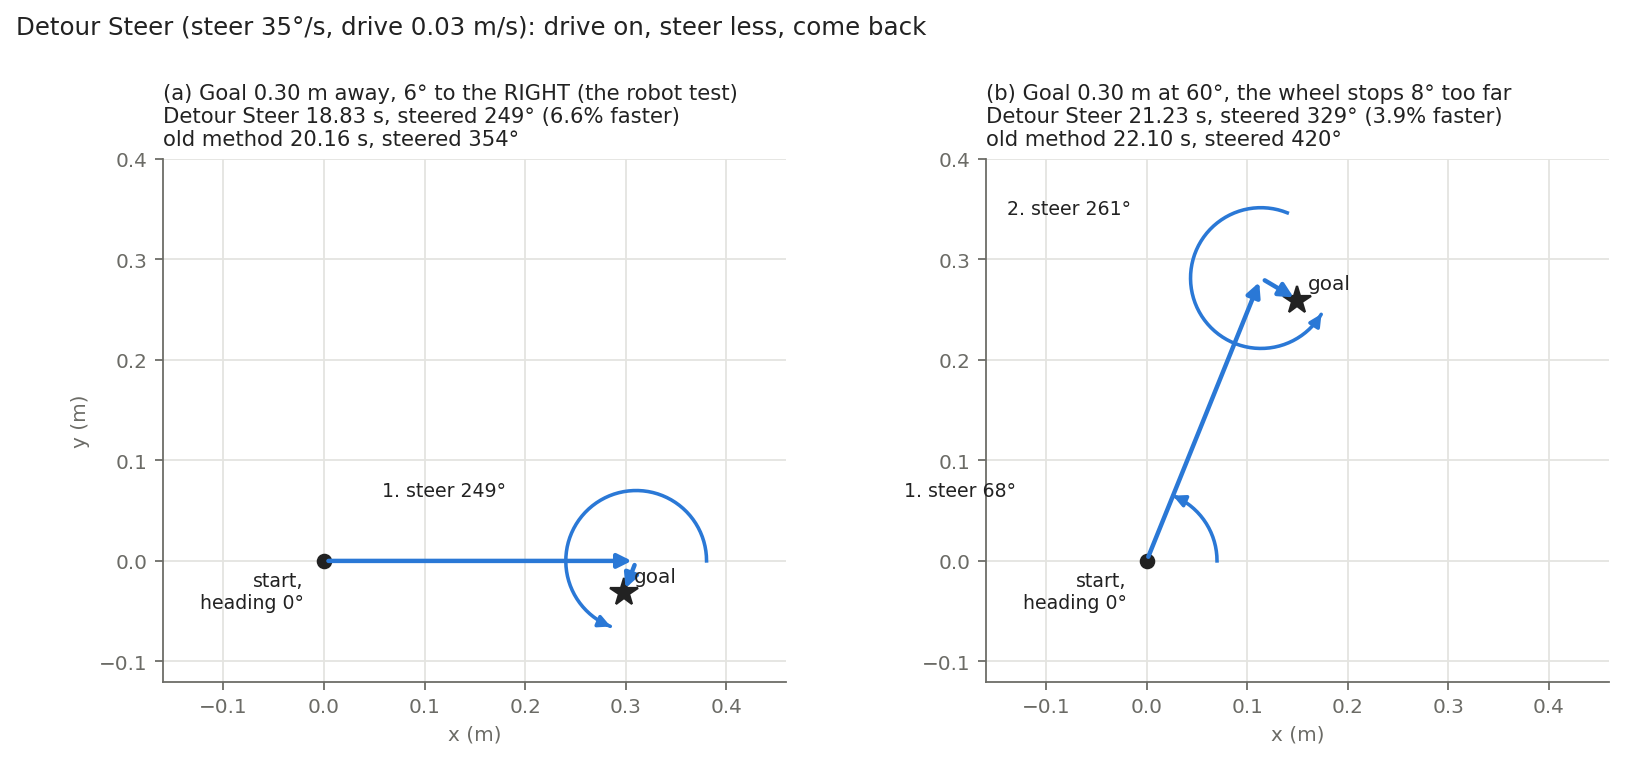
\includegraphics[width=0.86\linewidth]{sim_path.png}\end{center}
\noindent\rule{\linewidth}{1.1pt}\par

\vspace{4mm}
\Needspace*{100mm}
\noindent\rule{\linewidth}{1.1pt}\par\vspace{1.4mm}
\noindent\textbf{รูปที่ 2} ถ้าเป็นความเร็วอื่น: เวลาที่ประหยัดได้บนเป้า 5000 จุดชุดเดิม\par\vspace{1.4mm}
\noindent\rule{\linewidth}{0.5pt}\par\vspace{2mm}
\begin{center}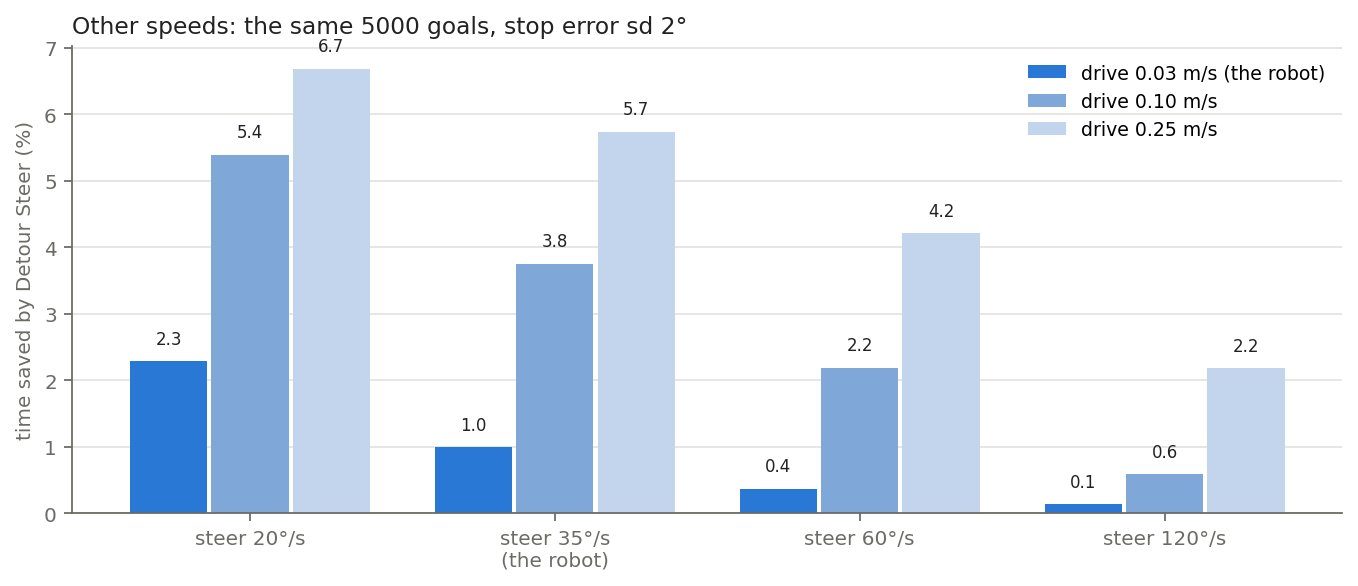
\includegraphics[width=0.80\linewidth]{sim_speeds.png}\end{center}
\noindent\rule{\linewidth}{1.1pt}\par


\Needspace*{90mm}
\noindent\rule{\linewidth}{1.1pt}\par\vspace{1.4mm}
\noindent\textbf{รูปที่ 3} ซิมเส้นทาง 2 เมตร / 7 ช่วง ที่ความเร็วของหุ่นจริง\par\vspace{1.4mm}
\noindent\rule{\linewidth}{0.5pt}\par\vspace{2mm}
\begin{center}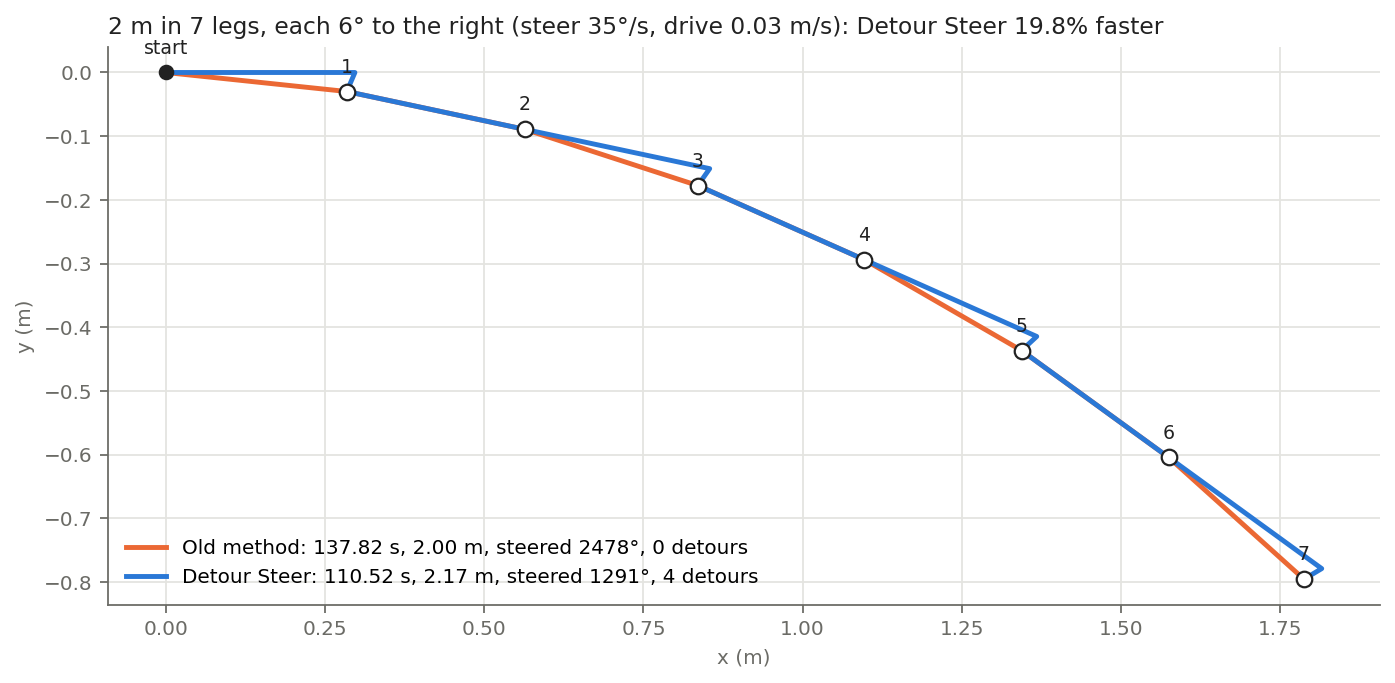
\includegraphics[width=0.92\linewidth]{sim_route_2m.png}\end{center}
\noindent\rule{\linewidth}{1.1pt}\par

\clearpage
\section*{ส่วนที่ 2 หุ่นจริง: ผลที่วัดได้ และซิมแบบใกล้เคียงหุ่นจริง}
{\small
\noindent\textbf{ผลบนหุ่นจริง} (\texttt{mor\_luam}: $v = 0.03$\,m/s, $\omega = 35^\circ$/s ซึ่งเป็นความเร็วเลี้ยวที่วัดได้,
$t_b = 0.2$\,s, $r_{goal} = 2.5$\,mm) งานเดียวกันทั้งสองวิธี: ก่อนเริ่มจับเวลา ล้อถูกหมุนไปทิศเริ่มต้นและนิ่งแล้ว
จากนั้นวางเป้าห่าง $d = 0.30$\,m ที่มุม $\varphi = 354^\circ$ จากทิศที่ล้อชี้อยู่จริง
หุ่นจับเวลาเองทุกรอบและวิ่งกลับจุดเริ่ม (ไม่จับเวลาขากลับ) ทำ 3 รอบ ลำดับ เดิม--Detour, Detour--เดิม, เดิม--Detour:
\begin{center}
\begin{tabular}{lrrr}
\toprule
รอบ & วิธีเดิม (s) & Detour Steer (s) & ประหยัด (s) \\
\midrule
1 & 24.17 & 20.83 & 3.34 \\
2 & 22.94 & 20.77 & 2.17 \\
3 & 23.36 & 22.33 & 1.03 \\
\midrule
เฉลี่ย & 23.49 & 21.31 & 2.18 (9.3\,\%) \\
\bottomrule
\end{tabular}
\end{center}
\noindent Detour Steer เร็วกว่าทั้ง 3 รอบ เลี้ยวน้อยลง 3.8\,s (8.5 เทียบ 12.4\,s) และวิ่งนานขึ้น 1.2\,s
(11.8 เทียบ 10.6\,s) แผนทำนายไว้ 18.8 เทียบ 20.2\,s แต่บนพื้นจริงต่างกันมากกว่า
เพราะวิธีเดิมที่หมุนเกือบรอบต้องแก้ทิศตอนท้ายมากกว่าด้วย ทั้ง 6 รอบหยุดห่างเป้าไม่เกิน 2.5\,mm

\medskip
\noindent\textbf{ทำไมหุ่นออกขวา (ทั้งสองวิธี)}
(1) มอเตอร์ตัวเดียวใช้ทั้งเลี้ยวและวิ่ง หุ่นจึงแก้ทิศระหว่างวิ่งไม่ได้ ความเบี่ยงสะสมจนต้องหยุดแล้วเล็งใหม่ (อัลกอริทึม 1.7)
(2) การเลี้ยวกับการวิ่งส่งผลต่อกันผ่านชุดเฟืองเดียวกัน แรงขับหมุนชุดล้อและเฟืองไปเล็กน้อย (ระหว่างวิ่ง มุม AS5600 เปลี่ยนไปเรื่อย ๆ และหน้าหุ่นหมุน)
และการเลี้ยวเกือบรอบทำให้ตัวหุ่นบิดตามประมาณ $4^\circ$
(3) ล้อลื่น พื้นไม่เรียบ และน้ำหนักตัวหุ่นไม่สมดุล
(4) หุ่นตั้งใจหยุดเลี้ยวก่อนถึงมุมประมาณ $2^\circ$ (ถ้าเกินต้องหมุนอีกเกือบรอบ)
หุ่นเลี้ยวทวนเข็ม การหยุดขาดจึงทำให้ล้อชี้เยื้องไปทางขวาของเป้าเล็กน้อย
รวมกันแล้วตัวหุ่นเบี่ยงประมาณ $3^\circ$ ระหว่างวิ่ง (วัดด้วย IMU) ทั้งสองวิธีออกขวาจากเส้น 1--3\,cm
แล้วการเล็งใหม่ก่อนถึงเป้า (เลี้ยวประมาณ $18^\circ$) ดึงกลับเข้าเป้า

\medskip
\noindent\textbf{ซิมต่างจากหุ่นจริงเท่าไร} เส้นทางที่ทำทั้งซิมและหุ่นจริงคือการทดสอบบนหุ่น
(เป้า 0.30\,m ที่ $354^\circ$ วิธีละ 3 รอบ) ซิมใช้ค่าที่วัดจากหุ่นจริง
($v = 0.03$\,m/s, $\omega = 35^\circ$/s, $t_b = 0.2$\,s, $r_{goal} = 2.5$\,mm):
\begin{center}
\begin{tabular}{lrrr}
\toprule
 & ซิม (s) & หุ่นจริง เฉลี่ย 3 รอบ (s) & ความคลาดเคลื่อน \\
\midrule
วิธีเดิม       & 20.16 & 23.49 & $-3.33$\,s ($-14.2\,\%$) \\
Detour Steer & 18.83 & 21.31 & $-2.48$\,s ($-11.6\,\%$) \\
เวลาที่ประหยัด & 1.33 (6.6\,\%) & 2.18 (9.3\,\%) & \\
\bottomrule
\end{tabular}
\end{center}
ซิมเร็วกว่าหุ่นจริง 11.6--14.2\,\% เพราะในซิมไม่มีการเบี่ยง ไม่มีล้อลื่น และไม่มีการหยุดเล็งใหม่
(ดูหัวข้อ ``ทำไมหุ่นออกขวา'') และซิมให้ผลประหยัดน้อยกว่าของจริง: หุ่นจริงประหยัด 9.3\,\% ซิม 6.6\,\%
เพราะวิธีเดิมที่หมุนเกือบรอบต้องแก้ทิศบนพื้นจริงมากกว่า

\smallskip
\noindent\textbf{ซิมแบบใกล้เคียงหุ่นจริง จากค่าที่วัดได้} log ของหุ่นเอง (ทุก 10\,ms; เลี้ยวใหญ่ 15 ครั้ง
เลี้ยวเล็ก 5 ครั้ง วิ่ง 23 ครั้ง, \texttt{tools/test\_out}) บอกว่าหุ่นเคลื่อนที่จริงอย่างไร ซิมสุ่มการเลี้ยวและการวิ่ง
แต่ละครั้งจากการกระจายที่วัดได้นี้ ทุกรอบจึงไม่เหมือนกัน (วิธีละ 1000 รอบ; ช่วง = 5--95\,\%):
\begin{itemize}\setlength\itemsep{0pt}
\item เวลาเลี้ยว (มอเตอร์ทำงาน) $= 0.90$\,s $+$ มุม$/37.8^\circ$/s กระจาย sd 0.19\,s (เลี้ยว $3$--$4^\circ$: 0.5--0.65\,s)
  ความเร็วไม่คงที่: ค่อย ๆ เร่ง วิ่งที่ 30--50$^\circ$/s แล้วช้าลงตอนท้าย
\item หลังเลี้ยวรอ 0.11\,s (วัดได้) บวกรอ IMU นิ่งอีกไม่เกิน 0.4\,s ในเฟิร์มแวร์ปัจจุบัน
\item ล้อตั้งใจหยุดขาด $2^\circ$ กระจาย $0.15^\circ$ (วัดได้)
\item ระหว่างวิ่ง ทิศที่หุ่นเคลื่อนที่หมุนไปทางขวา $14.4 \pm 14.5^\circ$/m: ตัวหุ่น $7.4 \pm 7.1^\circ$/m (IMU)
  บวกชุดล้อ $7.0 \pm 12.6^\circ$/m (AS5600) เพราะแรงขับหมุนชุดล้อและเฟือง
\item เล็งใหม่ก่อนถึงเป้า (อัลกอริทึม 1.7)
\item หมุนเกิน: ถ้าเลี้ยวเลยมุมต้องหมุนอีกเกือบรอบ ใน log 20 ครั้งไม่มีครั้งไหนหมุนเกิน แต่เกิดจริงบนหุ่น
  จึงทดสอบด้วยโอกาส $p$ ต่อการเลี้ยวหนึ่งครั้ง
\end{itemize}
\begin{center}
\begin{tabular}{lrr}
\toprule
 & วิธีเดิม (s) & Detour Steer (s) \\
\midrule
หุ่นจริง 3 รอบ           & 23.49 (22.94--24.17) & 21.31 (20.77--22.33) \\
ซิม, $p = 0$            & 23.95 (22.09--26.11), $+2.0\,\%$ & 18.42 (16.83--20.99), $-13.6\,\%$ \\
ซิม, $p = 3\,\%$        & 24.67 (22.15--33.94), $+5.0\,\%$ & 18.67 (16.73--21.93), $-12.4\,\%$ \\
ซิม, $p = 8\,\%$        & 26.11 (22.22--36.41), $+11.2\,\%$ & 18.99 (16.73--25.79), $-10.9\,\%$ \\
\bottomrule
\end{tabular}
\end{center}
ใช้แค่ค่าที่วัดได้ (ไม่ได้ปรับค่าใดเลย) วิธีเดิมตรงกับหุ่นจริงภายใน 2\,\% แต่ Detour Steer บนหุ่นจริงช้ากว่าซิม
ประมาณ 2.9\,s: Detour บนหุ่นจริงทุกรอบจบด้วยการเลี้ยวเล็ก ๆ อีกครั้งและวิ่งสั้น ๆ (รูปที่ 4 ช่วงชมพูและน้ำเงินท้ายสุด)
ซึ่งซิมไม่เกิด log ที่มีอยู่ไม่มีรอบ Detour จึงยังวัดสาเหตุไม่ได้ ถ้ามี log ของรอบ Detour จะปิดช่องว่างนี้ได้
ซิมนี้จึงให้ผลประหยัดเกินจริง (23\,\% เทียบ 9.3\,\%) และไม่ใช้อ้างตัวเลขของหุ่นจริง
การหมุนเกินทำให้วิธีเดิมช้าลง (เสียเกือบหนึ่งรอบต่อครั้ง) ส่วน Detour Steer เปลี่ยนการพลาดนั้นเป็นทางอ้อม
หน้าต่างซิมมีโหมดเดียวกัน (ช่อง ``แบบใกล้หุ่นจริง'') กดเริ่มแต่ละครั้งได้ 1 รอบสุ่มใหม่ และแสดงค่าเฉลี่ยกับช่วงจาก 1000 รอบ

\smallskip
\noindent\textbf{เส้นทาง 2 เมตร ในซิมแบบใกล้เคียงหุ่นจริง} เส้นทางนี้ทดสอบในซิมเท่านั้น ยังไม่ได้วิ่งบนหุ่นจริง
ในซิมจากค่าที่วัดได้ ($p = 0$, วิธีละ 1000 รอบ) ผลขึ้นกับระยะที่ถือว่าถึงจุด (\texttt{navTolM}) การทดสอบบนหุ่นใช้ 2.5\,mm:
\begin{center}
\begin{tabular}{lrrr}
\toprule
ระยะถึงจุด & วิธีเดิม (s) & Detour Steer (s) & ประหยัด \\
\midrule
2.5\,mm (เท่าที่ทดสอบ) & 154.6 (150.8--158.1) & 143.1 (132.1--148.2) & 7.4\,\% \\
1\,cm               & 150.5 (147.4--153.4) & 130.4 (105.5--142.7) & 13.4\,\% \\
2\,cm               & 149.7 (146.8--152.4) & 118.1 (80.7--139.9)  & 21.1\,\% \\
6\,cm               & 144.5 (133.4--148.7) & 108.0 (76.4--135.8)  & 25.3\,\% \\
\bottomrule
\end{tabular}
\end{center}
ที่ 2.5\,mm ทั้งสองวิธีเสียเวลามากกับการแก้ทิศเล็ก ๆ ที่จุดทั้ง 7 จุด และเพราะซิมเร็วเกินจริงสำหรับ Detour Steer
ในการทดสอบ 0.30\,m ตัวเลขประหยัดเหล่านี้จึงเป็นค่าสูงสุด ขากลับจุดเริ่ม (ประมาณ 1.96\,m) ไม่นับเวลา

\medskip
\noindent\textbf{สรุปส่วนที่ 2} บนหุ่นจริง Detour Steer เร็วกว่าทั้ง 3 รอบ: 21.31\,s เทียบ 23.49\,s (9.3\,\%)
ผลที่วัดได้นี้คือผลที่เชื่อถือได้ หุ่นจริงช้ากว่าแบบจำลองอุดมคติ 11.6--14.2\,\% เพราะการเบี่ยง ชุดล้อที่หมุนเอง
ล้อลื่น และการหยุดเล็งใหม่ ซิมที่สร้างจาก log ของหุ่นอย่างเดียวตรงกับวิธีเดิมภายใน 2\,\% แต่เร็วเกินจริง
สำหรับ Detour Steer ประมาณ 2.9\,s (การแก้ทิศตอนท้ายหนึ่งครั้งที่ซิมยังไม่เกิด) เส้นทาง 2 เมตรทดสอบในซิมเท่านั้น
}

\vspace{4mm}
\Needspace*{135mm}
\noindent\rule{\linewidth}{1.1pt}\par\vspace{1.4mm}
\noindent\textbf{รูปที่ 4} ผล 3 รอบบนหุ่นจริง จากข้อมูลที่หุ่นบันทึกเอง\par\vspace{1.4mm}
\noindent\rule{\linewidth}{0.5pt}\par\vspace{2mm}
\begin{center}
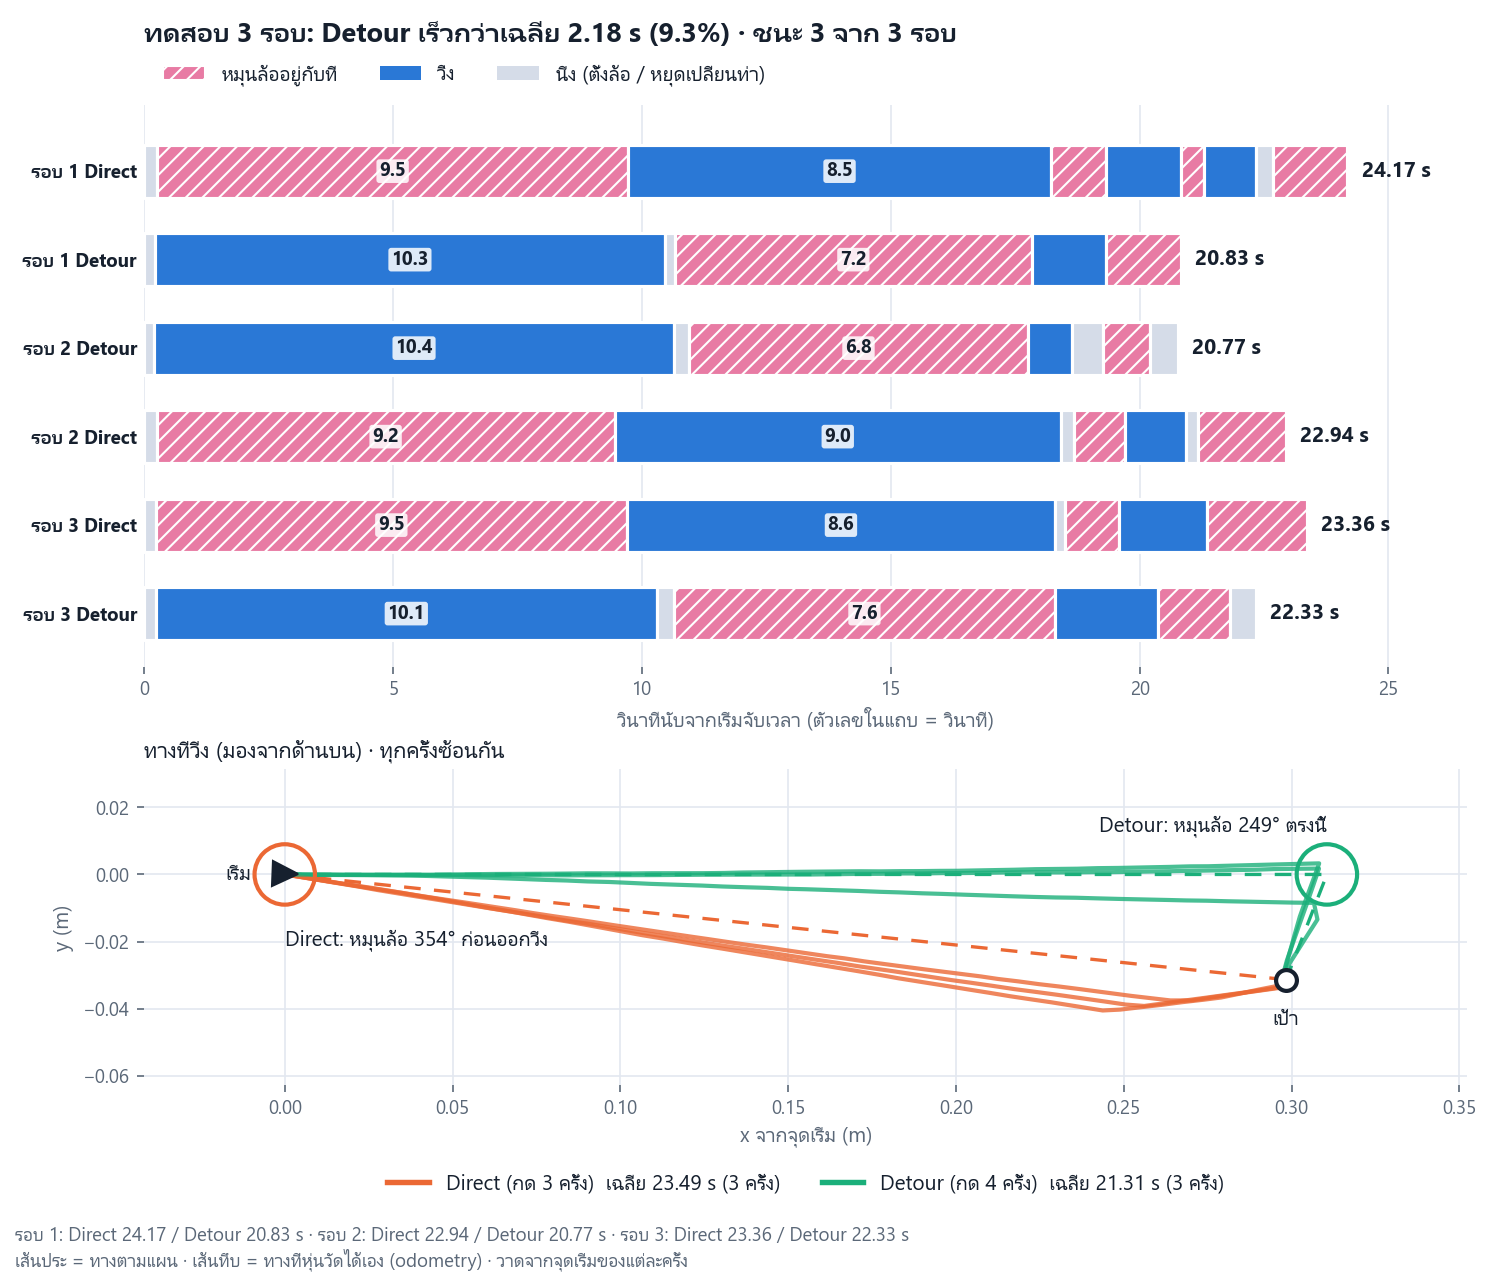
\includegraphics[width=0.93\linewidth]{robot_3rounds.png}
\end{center}
{\small
\noindent\textbf{บน:} สิ่งที่แต่ละรอบทำตามเวลา (ลายชมพู = เลี้ยวอยู่กับที่, น้ำเงิน = วิ่ง, เทา = นิ่ง)
วิธีเดิมเลี้ยวอยู่กับที่ก่อน $\approx 9.4$\,s แล้วค่อยวิ่ง ส่วน Detour Steer วิ่งทันทีและเลี้ยวน้อยกว่าในภายหลัง
\textbf{ล่าง:} เส้นทางที่หุ่นวัดได้ (odometry) ทั้ง 6 รอบจากจุดเริ่มเดียวกัน มองจากด้านบน เส้นประ = แผน
(หุ่นเลี้ยวทวนเข็ม ในรูปนี้เป้าจึงอยู่ทางขวา)\par}
\vspace{1mm}
\noindent\rule{\linewidth}{1.1pt}\par



\clearpage
\section*{ภาคผนวก ก. โค้ดและ Git}
โค้ดทั้งหมดของอัลกอริทึมนี้ (ตัววางแผน Python, ซิม, เฟิร์มแวร์บนหุ่น และรายงานนี้) อยู่บน Git:

\begin{center}
\large\url{https://github.com/Mannaja78520/mor_luam} \quad {\normalsize(branch \texttt{main})}
\end{center}

\noindent\textbf{วิดีโอการทำงานของหุ่น:}
\begin{center}
\url{https://drive.google.com/drive/folders/11qOM6UoeH2c4nEuM0a0JO6eXTnr0eDud}
\end{center}
\noindent{\small คลิปนี้เป็นการทำงานของหุ่นแบบ synchronize
ไม่มีคลิปของการเปรียบเทียบ Detour Steer กับวิธีเดิม (Direct)
ผลการเปรียบเทียบดูได้จากข้อมูลที่หุ่นบันทึกเองในรูปที่ 4 และตารางผลบนหุ่นจริง}\par\medskip

\noindent\textbf{อัลกอริทึมตัดสินใจอยู่ที่ไหน}
\begin{itemize}
\item \texttt{algorithm\_sim/detour\_steer.py} -- ตัววางแผนต้นแบบ ตรวจทฤษฎีบท T1--T4 benchmark และสร้างรูป
\item \texttt{algorithm\_sim/sim\_detour\_steer.py}, \texttt{sim\_detour\_only.py} -- หน้าต่างซิมบนคอม
\item \texttt{firmware/src/algorithm/DetourSteer.\{h,cpp\}} -- ตัววางแผนเดียวกันในภาษา C++ บน ESP32
\item \texttt{firmware/src/nav/WaypointRunner.cpp} -- สั่งหุ่นวิ่งตามแผนทีละช่วง;
\texttt{FinalApproach.h} และ \texttt{SteerApproach.h} -- อัลกอริทึม 1.6 และ 1.7
\end{itemize}

\noindent\textbf{ดาวน์โหลดโค้ดและรันซิม (ไม่ต้องใช้ Docker)}
\begin{lstlisting}[numbers=none]
git clone https://github.com/Mannaja78520/mor_luam.git
cd mor_luam/algorithm_sim
pip install matplotlib
python detour_steer.py --no-bench      # theorem checks T1-T4 + figures
python sim_detour_steer.py             # old method vs Detour Steer
python -m unittest test_current_robot
\end{lstlisting}

\noindent\textbf{Build และอัปโหลดเฟิร์มแวร์ลงหุ่น (แนะนำติดตั้งแบบ Docker)}
\begin{lstlisting}[numbers=none]
docker\mor_luam.bat fw-build              # Windows, Docker Desktop running
docker\mor_luam.bat fw-flash -Port COM9   # first time, over USB
docker\mor_luam.bat fw-ota -Host <IP>     # later, over Wi-Fi
./docker/mor_luam.sh fw-build             # Ubuntu, same commands
\end{lstlisting}
วิธีติดตั้งทีละขั้น: \texttt{docs/INSTALL\_TH.md} ใน repository

% =========================================================== Code ===========
\clearpage
\subsection*{ก.1 ตัววางแผนใน Python (\texttt{algorithm\_sim/detour\_steer.py})}
\lstinputlisting[language=Python,firstline=247,lastline=305,firstnumber=247]{../detour_steer.py}

\subsection*{ก.2 ตัววางแผนบนหุ่น (\texttt{firmware/src/algorithm/DetourSteer.h})}
\lstinputlisting[language=C++]{../../firmware/src/algorithm/DetourSteer.h}

\subsection*{ก.3 ตัววางแผนบนหุ่น (\texttt{firmware/src/algorithm/DetourSteer.cpp})}
\lstinputlisting[language=C++]{../../firmware/src/algorithm/DetourSteer.cpp}
\end{document}
